\documentclass[12pt, t]{beamer}

%------------------------------------------------------------------------------
% configuration
%------------------------------------------------------------------------------
\RequirePackage{etex}
\usepackage{../../themes/dbt}
\usepackage{catchfilebetweentags}

\setbeameroption{hide notes}
\setbeamertemplate{caption}{\raggedright\insertcaption\par}

\graphicspath{{images/}}

% a few macros
\newcommand{\bi}{\begin{itemize}}
\newcommand{\ei}{\end{itemize}}
\newcommand{\ig}{\includegraphics}
\newcommand{\myhref}[1]{\href{#1}{\tt \tiny #1}}
\newcommand{\incnote}[1]{\note{\ExecuteMetaData[notes.tex]{#1}}}
\newcommand{\src}[2]{\vspace{-10pt}\caption{\href{#1}{\centering \tt \tiny [#2]}}}

%------------------------------------------------------------------------------
% title
%------------------------------------------------------------------------------
% slide
\title{Systèmes d'exploitation pour l'embarqué}
\subtitle{UV 5.2 - Exécution et Concurrence}

\author{\href{}{Paul Blottière}}
\institute{
    \href{http://www.ensta-bretagne.fr/}{ENSTA Bretagne} \\[2pt]
    \href{}{\tt \scriptsize 24 Novembre 2015}
}
\date{
    \href{https://github.com/pblottiere}{\tt \scriptsize https://github.com/pblottiere} \\[2pt]
    %\href{blottiere.paul@gmail.com}{\tt \scriptsize blottiere.paul@gmail.com}
}

% info
\begin{document}

{
\setbeamertemplate{footline}{} % no page number here
\frame{
    \titlepage
    \incnote{title}
} }

%------------------------------------------------------------------------------
% amélioration continue
%------------------------------------------------------------------------------
\begin{frame}{Amélioration continue}
    \subt{Contributions}
    \vspace{12pt}

    \begin{center}
    
\includegraphics[scale=0.7]{github.png}
    \end{center}

    \bi
    \itemsep12pt
    \item Dépôt du cours : \href{https://github.com/pblottiere/embsys}{\tt \scriptsize https://github.com/pblottiere/embsys}

    \onslide<2->{
        \item Souhaits d'amélioration, erreurs, idées de TP, ... : ouverture d'Issues (avec le bon label!)
        \item Apports de corrections : Pull Request
        \ei
    }
\end{frame}

%------------------------------------------------------------------------------
% exam
%------------------------------------------------------------------------------
%\begin{frame}{Projet}
%    \vspace{10pt}
%    \begin{figure}
%        \centering
%        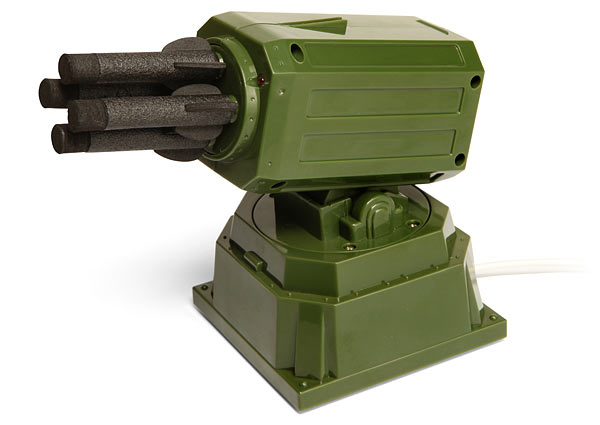
\includegraphics[scale=0.4]{rocket_launcher.jpg}
%    \end{figure}
%\end{frame}

%<**lecture_content>
%------------------------------------------------------------------------------
% lecture
%------------------------------------------------------------------------------
\begin{frame}[plain,c]
    \centering
    \huge\textcolor{title}{IPC et programmation réseau}
\end{frame}

%------------------------------------------------------------------------------
% plan
%------------------------------------------------------------------------------
\begin{frame}{Plan}
    \subt{}
    \vspace{10pt}

    \begin{enumerate}
        \itemsep12pt
        \item Descripteur de fichier
        \item IPC : qu'est-ce?
        \item Pipe
        \item File de messages
        \item Mémoire partagée
        \item Sémaphore
        \item Programmation réseau
        \item Multiplexage d'entrées
    \end{enumerate}

    \note {
    }
\end{frame}

%------------------------------------------------------------------------------
% fd1
%------------------------------------------------------------------------------
\begin{frame}{Descripteur de fichier (1)}
    \subt{Généralités}
    \vspace{15pt}

    File descriptor : entier compris entre 0 et OPEN\_MAX.

    \onslide<2->{
        \vspace{15pt}
        Trois descripteurs réservés :
        \bi
        \itemsep6pt
        \item 0 : STDIN\_FILENO
        \item 1 : STDOUT\_FILENO
        \item 2 : STDERR\_FILENO
        \ei
    }

    \onslide<3->{
        \vspace{15pt}
        Un flux de type {\textbf{FILE *}} est associé aux descripteurs de fichier
        par défaut :
        \bi
        \itemsep6pt
        \item stdin
        \item stdout
        \item stderr
        \ei
    }

    \incnote{fd1}
\end{frame}

%------------------------------------------------------------------------------
% fd2
%------------------------------------------------------------------------------
\begin{frame}{Descripteur de fichier (2)}
    \subt{/proc/<PID>/fd/}

    \vspace{10pt}
    Une liste de tous les file descriptors d'un processus est disponible dans
    le {\textbf{/proc}} :

    \vspace{10pt}
    \begin{figure}
        \centering
        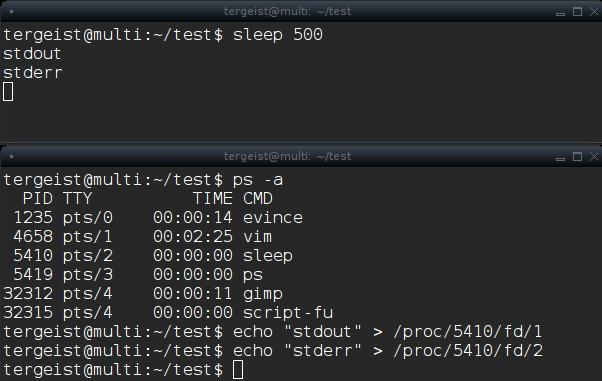
\includegraphics[scale=0.55]{fd_proc.png}
    \end{figure}

\end{frame}

%------------------------------------------------------------------------------
% fd3
%------------------------------------------------------------------------------
\begin{frame}{Descripteur de fichier (3)}
    \subt{Exemple (fd.c)}

    \lstinputlisting[label=samplecode, basicstyle=\tiny]{code/fd.c}

    \vspace{-15pt}
    \begin{figure}
        \centering
        \vspace{-30pt}
        \hspace{80pt}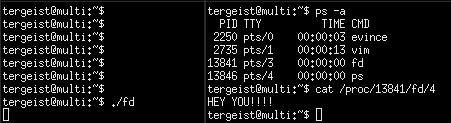
\includegraphics[scale=0.55]{fd.png}
    \end{figure}
\end{frame}

%------------------------------------------------------------------------------
% ipc1
%------------------------------------------------------------------------------
\begin{frame}{IPC : qu'est-ce?}
    \subt{Principe}

    \vspace{15pt}
    Entre threads, la communication est simple : données partagées au sein
    du même espace mémoire.

    \onslide<2->{
        \vspace{15pt}
        Dans le cas de communication entre processus, des mécanismes sont
        nécessaires!
    }

    \onslide<2->{
        \vspace{15pt}
        Ce sont les Inter Process Communication (définis par SUSv4) :
        \bi
        \itemsep12pt
        \item pipe
        \item file de messages
        \item mémoire partagée (et sémaphore pour la synchronisation)
        \ei
    }

\end{frame}

%------------------------------------------------------------------------------
% pipe1
%------------------------------------------------------------------------------
\begin{frame}{Pipe (1)}
    \subt{Définition}

    \vspace{10pt}
    Moyen de communication unidirectionnel.

    \onslide<2->{
        \vspace{10pt}
        Deux extrémités représentées par des file descriptors :
        \vspace{8pt}
        \begin{figure}
            \centering
            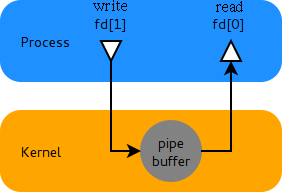
\includegraphics[scale=0.6]{pipe.png}
            \src{http://hzqtc.github.io/2012/07/linux-ipc-with-pipes.html}{Pipe}
        \end{figure}
    }

    \vspace{-5pt}
    \onslide<3->{
        => comme les fd doivent être connus pour l'écriture  et la lecture, les
        pipe sont utilisables avec les threads ou les processus dupliqués (fork)!
    }

\end{frame}

%------------------------------------------------------------------------------
% pipe2
%------------------------------------------------------------------------------
\begin{frame}[fragile]{Pipe (2)}
    \subt{Comment?}

    \vspace{15pt}
    Cinq fonctions :
    \vspace{8pt}
    \bi
    \itemsep12pt
    \item {\textbf{pipe}} : création du tube
    \item {\textbf{write}} : écriture dans le tube
    \item {\textbf{read}} : lecture des données
    \item {\textbf{close}} : fermeture du tube
    \ei

    \onslide<2->{
        \vspace{15pt}
        => une écriture dans un pipe dont l'extrémité est fermée échoue!
    }

\end{frame}

%------------------------------------------------------------------------------
% pipe3
%------------------------------------------------------------------------------
\begin{frame}{Pipe (3)}
    \subt{pipe.c}

    \lstinputlisting[label=samplecode, basicstyle=\tiny]{code/pipe.c}

    \onslide<2->{
        \begin{figure}
            \vspace{-40pt}
            \hspace{50pt}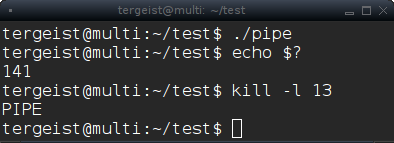
\includegraphics[scale=0.55]{pipe_error.png}
        \end{figure}

        \begin{figure}
            \vspace{-100pt}
            \hspace{220pt}
\includegraphics[scale=0.4]{tux_why.png}
        \end{figure}
    }

\end{frame}

%------------------------------------------------------------------------------
% pipe4
%------------------------------------------------------------------------------
\begin{frame}{Pipe (4)}
    \subt{Named pipe}

    \vspace{15pt}
    Pour faire communiquer des processus distincts (n'ayant pas accès au file
    descriptor du tube), il existe des {\textbf{tubes nommés}}.

    \onslide<2->{
        \vspace{15pt}
        Contrairement au tube simple résidant en mémoire, un tube nommé possède
        une représentation au sein du système de fichiers.

        \vspace{5pt}
        \begin{figure}
            \centering
            
\includegraphics[scale=0.17]{tux_pipe.png}
        \end{figure}
    }

\end{frame}

%------------------------------------------------------------------------------
% pipe5
%------------------------------------------------------------------------------
\begin{frame}[fragile]{Pipe (5)}
    \subt{Named pipe}

    \vspace{10pt}
    Six fonctions :
    \vspace{5pt}
    \bi
    \itemsep6pt
    \item {\textbf{mkfifo}} : création du fichier représentant le tube
    \item {\textbf{open}} : ouverture du tube
    \item {\textbf{write}} : écriture de données dans le tube
    \item {\textbf{read}} : lecture des données
    \item {\textbf{close}} : fermeture du tube
    \item {\textbf{unlink}} : suppression du fichier représentant le tube
    \ei

    \vspace{15pt}
    \begin{lstlisting}
#include <sys/stat.h>

int mkfifo(const char * pipe_name, mode_t mode);
    \end{lstlisting}

\end{frame}

%------------------------------------------------------------------------------
% pipe6
%------------------------------------------------------------------------------
\begin{frame}{Pipe (6)}
    \subt{named\_pipe.c}

    \vspace{10pt}
    \lstinputlisting[label=samplecode, basicstyle=\tiny]{code/named_pipe.c}

    \onslide<2->{
        \begin{figure}
            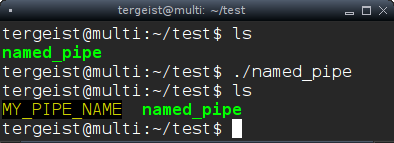
\includegraphics[scale=0.55]{named_pipe.png}
        \end{figure}
    }

\end{frame}

%------------------------------------------------------------------------------
% msg1
%------------------------------------------------------------------------------
\begin{frame}{File de messages (1)}
    \subt{Différence avec les tubes}

    \vspace{15pt}
    La communication par tubes se fait par l'intermédiaire de flux : la taille
    des données peut être variable entre chaque écriture/lecture.

    \onslide<2->{
        \vspace{15pt}
        La communication par file de messages se fait par passage de messages de
        taille fixe avec des niveaux de priorité!

        \vspace{15pt}
        \begin{figure}
            \centering
            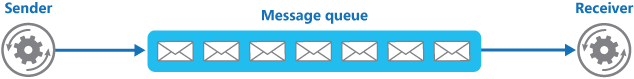
\includegraphics[scale=0.5]{msgq.png}
            \src{https://msdn.microsoft.com/en-us/library/dn589781.aspx}{Message Queue}
        \end{figure}
    }

    \incnote{msg1}

\end{frame}

%------------------------------------------------------------------------------
% msg2
%------------------------------------------------------------------------------
\begin{frame}[fragile]{File de messages (2)}
    \subt{Comment?}

    \vspace{10pt}
    Les cinq appels système principaux :
    \vspace{5pt}
    \bi
    \itemsep8pt
    \item {\textbf{mq\_open}} : ouverture d'une file
    \item {\textbf{mq\_close}} : fermeture de la file
    \item {\textbf{mq\_unlink}} : destruction de la file
    \item {\textbf{mq\_send}} : envoie d'un message dans la file
    \item {\textbf{mq\_receive}} : réception d'un message
    \ei

    \vspace{10pt}
    \begin{lstlisting}
#include <mqueue.h>

mqd_t mq_send(mqd_t mq, const char * msg,
              size_t size_msg,
              unsigned int priority);
    \end{lstlisting}

\end{frame}

%------------------------------------------------------------------------------
% msg3
%------------------------------------------------------------------------------
\begin{frame}{File de messages (3)}
    \subt{mq\_server.c / mq\_client.c}

    \lstinputlisting[label=samplecode, basicstyle=\tiny]{code/mq_server.c}

    \vspace{-90pt}
    \begin{figure}
        \hspace{80pt} 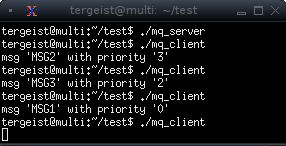
\includegraphics[scale=0.45]{mq.png}
    \end{figure}

\end{frame}

%------------------------------------------------------------------------------
% shm1
%------------------------------------------------------------------------------
\begin{frame}{Mémoire partagée (1)}
    \subt{Principe}

    \vspace{10pt}
    Shared memory : segment de mémoire accessible en lecture / écriture par
    plusieurs processus et persistant jusqu'au {\textbf{reboot}} de la
    machine.

    \vspace{15pt}
    \begin{figure}
        \centering
        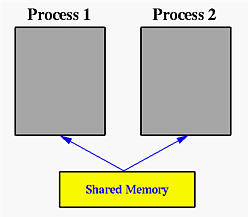
\includegraphics[scale=0.5]{shm.jpg}
        \src{http://www.csl.mtu.edu/cs4411.ck/www/NOTES/process/shm/what-is-shm.html}{Shared memory}
    \end{figure}

\end{frame}

%------------------------------------------------------------------------------
% shm2
%------------------------------------------------------------------------------
\begin{frame}[fragile]{Mémoire partagée (2)}
    \subt{Les appels système}

    \vspace{15pt}
    Quatre appels système :
    \vspace{5pt}
    \bi
    \itemsep8pt
    \item {\textbf{shm\_open}} : ouverture du segment mémoire
    \item {\textbf{ftruncate}} : dimensionnement du segment
    \item {\textbf{mmap}} : projection de la structure de données sur le segment
    \item {\textbf{shm\_unlink}} : destruction du segment
    \ei

    \vspace{10pt}
    \begin{lstlisting}
int shm_open(const char * name, int flags,
             mode_t mode);
    \end{lstlisting}

\end{frame}

%------------------------------------------------------------------------------
% shm3
%------------------------------------------------------------------------------
\begin{frame}{Mémoire partagée (3)}
    \subt{shm\_server.c / shm\_drinker.c}

    \begin{figure}
        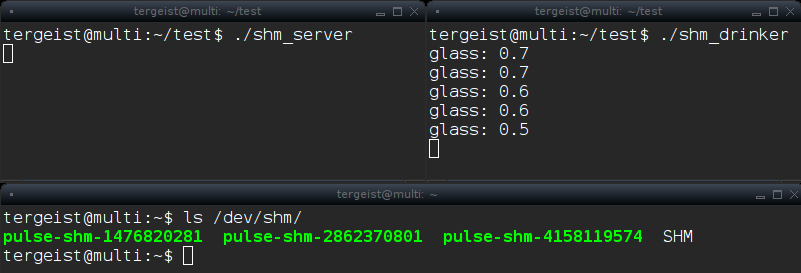
\includegraphics[scale=0.5]{shm.png}
    \end{figure}

    => mais peut avoir des problèmes d'accès concurrent!

\end{frame}

%------------------------------------------------------------------------------
% sem1
%------------------------------------------------------------------------------
\begin{frame}{Sémaphore (1)}
    \subt{Principe}

    \vspace{15pt}
    Les communications multiprocessus à travers la mémoire partagée peut
    conduire à des incohérences dans les données si les accès ne sont pas
    synchronisés.

    \vspace{15pt}
    => contrôle d'accès aux ressources critiques via les sémaphores!

    \onslide<2->{
        \vspace{20pt}
        On peut aussi gérer le nombre d'accès simultanés maximum autorisé.
    }
\end{frame}

%------------------------------------------------------------------------------
% sem2
%------------------------------------------------------------------------------
\begin{frame}{Sémaphore (2)}
    \subt{flags levés / baissés}

    \vspace{12pt}
    L'accès à la donnée :
    \vspace{5pt}
    \begin{enumerate}
        \itemsep8pt
        \item un processus attend que le flag soit levé (ressource disponible)
        \item le processus baisse le flag
        \item le processus utilise la ressource protégée
        \item le processus lève le flag pour indiquer qu'elle est disponible
        \item le kernel réveille les autres processus en attente
    \end{enumerate}
\end{frame}

%------------------------------------------------------------------------------
% sem3
%------------------------------------------------------------------------------
\begin{frame}[fragile]{Sémaphore (3)}
    \subt{versus mutex}

    \vspace{15pt}
    Mutex : surtout utilisé dans les applications multithreads (protection
    d'accès d'une section de code ne pouvant pas être exécutée par plus d'un
    thread).

    \vspace{15pt}
    Sémaphore : surtout utilisé pour les communications multiprocessus.

    \vspace{15pt}
    Mutex = Sémaphore local avec un nombre de clé de 1 (sémaphore binaire)

    \vspace{10pt}
    \begin{lstlisting}
sem_init(&mutex, 0, 1);
    \end{lstlisting}
\end{frame}

%------------------------------------------------------------------------------
% sem4
%------------------------------------------------------------------------------
\begin{frame}{Sémaphore (4)}
    \subt{Sémaphore nommé}

    \vspace{10pt}
    De même que pour les tubes, un nom peut être associé au sémaphore
    pour permettre à d'autres processus de l'utiliser!

    \vspace{10pt}
    \onslide<2->{
        Les sept appels système :
        \bi
        \itemsep5pt
        \item {\textbf{sem\_init}} : initialisation du sémaphore
        \item {\textbf{sem\_open}} x 2 : deux prototypes d'ouverture
                                        (créateur/utilisateur)
        \item {\textbf{sem\_close}} : fermeture du sémaphore
        \item {\textbf{sem\_unlink}} : destruction du sémaphore
        \item {\textbf{sem\_wait}} : attente bloquante du sémaphore
        \item {\textbf{sem\_post}} : relache le sémaphore
        \ei
    }

\end{frame}

%------------------------------------------------------------------------------
% net1
%------------------------------------------------------------------------------
\begin{frame}{Programmation réseau (1)}
    \subt{Les couches}

    \vspace{15pt}
    \begin{figure}
        \centering
        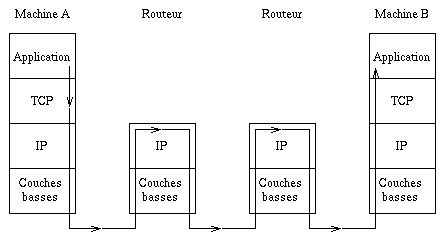
\includegraphics[scale=0.9]{layers.png}
        \src{http://www.grima.be/site/uploads/tlp/export/html-doc/tlp.html}{Les couches pour TCP / UDP}
    \end{figure}

\end{frame}

%------------------------------------------------------------------------------
% net2
%------------------------------------------------------------------------------
\begin{frame}{Programmation réseau (2)}
    \subt{Matériels et MAC}

    \vspace{8pt}
    Les principaux éléments d'un réseau :
    \bi
    \itemsep8pt
    \item {\textbf{hub}} : envoie toutes les données à toutes les machines
    \item {\textbf{switch}} : distribue les données aux machines destinataires
    \item {\textbf{routeur}} : liaison entre sous réseaux
    \ei

    \onslide<2->{
        \vspace{8pt}
        Les cartes Ethernet sont représentées par un identificateur unique
        appelé adresse MAC (Medium Access Control) :
        \vspace{5pt}
        \bi
        \itemsep5pt
        \item 24 premiers bits : numéro constructeur
        \item 24 derniers bits : numéro attribué par le constructeur
        \ei
    }

\end{frame}

%------------------------------------------------------------------------------
% net3
%------------------------------------------------------------------------------
\begin{frame}{Programmation réseau (3)}
    \subt{Internet Protocol}

    \vspace{8pt}
    Pour permettre la communication entre machines de sous réseaux différents,
    le protocole IP est utilisé!

    \vspace{8pt}
    Les adresses IP sont représentées sur 4 octets.

    \onslide<2->{
        \vspace{8pt}
        Adress Resolution Protocol : trouver l'adresse MAC d'une machine
        distante dont on ne connaît que l'adresse IP.

        \vspace{8pt}
        \begin{figure}
            \centering
            
\includegraphics[scale=0.35]{tux_wifi.png}
        \end{figure}
    }

\end{frame}

%------------------------------------------------------------------------------
% net4
%------------------------------------------------------------------------------
\begin{frame}{Programmation réseau (4)}
    \subt{TCP / UDP et diffusion}

    \vspace{8pt}
    Transmission Control Protocol (TCP) :
    \bi
    \item mode connecté : contrôle de flux, acquittement
    \item fiable : les données arrivent dans l'ordre (répétées si perdues)
    \ei

    \onslide<2->{
        \vspace{8pt}
        User Datagram Protocol (UDP) :
        \bi
        \item non connecté : pas d'acquittement
        \item non fiable : données non répétées si perdues
        \ei
    }

    \onslide<3->{
        \vspace{8pt}
        Diffusion :
        \bi
        \item unicast : envoie d'un message à une IP de classe A, B ou C
                        spécifique
        \item broadcast : envoie d'un message à toutes les IP
        \item multicast : envoie d'un message à toutes les IP de classe
                          D d'un groupe multicast
        \ei
    }

\end{frame}

%------------------------------------------------------------------------------
% net5
%------------------------------------------------------------------------------
\begin{frame}{Programmation réseau (5)}
    \subt{Port}

    \vspace{10pt}
    Plusieurs applications sont disponibles sur un seul serveur. Pour discuter
    de manière particulière avec une application, un numéro de port est
    donc nécessaire en plus de l'adresse IP.

    \vspace{10pt}
    Par exemple :
    \vspace{5pt}
    \bi
    \item ftp : 21
    \item ssh : 22
    \item http : 80
    \ei

    \vspace{-15pt}
    \begin{figure}
        \centering
        
\includegraphics[scale=0.5]{socket.png}
    \end{figure}

\end{frame}

%------------------------------------------------------------------------------
% net6
%------------------------------------------------------------------------------
\begin{frame}{Programmation réseau (6)}
    \subt{Les commandes utiles}

    \vspace{15pt}
    \bi
    \itemsep12pt
    \item {\textbf{ifconfig}} : configuration d'une interface réseau
    \item {\textbf{netstat}} : affiche les connexions réseaux, les ports
                               ouverts, ... (machine locale)
    \item {\textbf{nmap}} : scanneur de port, exploration du réseau
    \item {\textbf{ssh}} : connexion sur machine distante
    \item {\textbf{wireshark}} : analyseur réseau
    \item ftp, telnet, tcpdump, route, traceroute, ...
    \ei

    \myhref{https://debian-handbook.info/browse/fr-FR/stable/sect.network-diagnosis-tools.html}

\end{frame}

%------------------------------------------------------------------------------
% net7
%------------------------------------------------------------------------------
\begin{frame}{Programmation réseau (7)}
    \subt{Les sockets}

    \vspace{15pt}
    Tube permettant de faire dialoguer des machines distantes via le réseau IP.

    \onslide<2->{
        \vspace{10pt}
        Pour chaque socket, on doit indiquer :
        \bi
        \itemsep12pt
        \item Le domaine : IPv4, IPv6 ou local
        \item Le protocole : UDP / TCP
        \item Le port : int
        \ei
    }

    \onslide<3->{
        \vspace{15pt}
        Un socket est manipulé via un file descriptor.
    }

\end{frame}

%------------------------------------------------------------------------------
% net8
%------------------------------------------------------------------------------
\begin{frame}{Programmation réseau (8)}
    \subt{Appels système}

    \vspace{10pt}
    Côté client TCP :
    \bi
    \item {\textbf{socket}} : création du socket
    \item {\textbf{connect}} : connexion à un socket (adresse / port)
    \item {\textbf{send / recv}} : discussion
    \item {\textbf{close}} : fermeture du socket
    \ei

    \onslide<2->{
        \vspace{10pt}
        Côté serveur TCP :
        \bi
        \item {\textbf{socket}} : création du socket
        \item {\textbf{bind}} : assigne adresse/port au socket
        \item {\textbf{listen}} : attend des connexions
        \item {\textbf{accept}} : accepte une connexion (bloquant)
        \item {\textbf{send / recv}} : discussion
        \item {\textbf{close}} : fermeture du socket
        \ei
    }

\end{frame}

%------------------------------------------------------------------------------
% net9
%------------------------------------------------------------------------------
\begin{frame}{Programmation réseau (9)}
    \subt{Appels système}

    \vspace{10pt}
    Côté client UDP :
    \bi
    \item {\textbf{socket}} : création du socket
    \item {\textbf{sendto / recvfrom}} : discussion
    \item {\textbf{close}} : fermeture du socket
    \ei

    \vspace{20pt}
    \onslide<2->{
        Côté serveur UDP :
        \bi
        \item {\textbf{socket}} : création du socket
        \item {\textbf{bind}} : assigne adresse/port au socket
        \item {\textbf{recvfrom / sendto}} : discussion
        \item {\textbf{close}} : fermeture du socket
        \ei
    }

\end{frame}

%------------------------------------------------------------------------------
% mult1
%------------------------------------------------------------------------------
\begin{frame}{Multiplexage d'entrées (1)}
    \subt{Pourquoi?}

    \vspace{15pt}
    Dans un système communiquant, un même processus doit généralement gérer
    l'arrivée et l'envoi d'informations à travers plusieurs canaux de type
    différents.

    \onslide<2->{
        \vspace{15pt}
        \begin{figure}
            \centering
            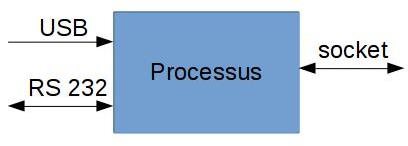
\includegraphics[scale=0.5]{mult.jpg}
        \end{figure}

        \vspace{15pt}
        => l'appel système {\textbf{select}} est utilisé pour le multiplexage!
    }

\end{frame}

%------------------------------------------------------------------------------
% mult2
%------------------------------------------------------------------------------
\begin{frame}{Multiplexage d'entrées (2)}
    \subt{Concept}

    \vspace{15pt}
    Étapes du multiplexage :
    \begin{enumerate}
    \itemsep8pt
    \item on indique au kernel les fd que je souhaite écouter
    \item tant que rien ne se passe, attente passive (pas de consommation CPU)
    \item quand une donnée est disponible, le kernel réveil le processus
    \item le processus regarde quel fd est prêt
    \item les données sont lues
    \item puis on retourne dans l'état d'attente passive jusqu'à la prochaine
          fois
    \end{enumerate}

\end{frame}

%------------------------------------------------------------------------------
% mult3
%------------------------------------------------------------------------------
\begin{frame}{Multiplexage d'entrées (3)}
    \subt{Les appels systèmes}

    \vspace{15pt}
    Cinq appels système principaux :
    \vspace{5pt}
    \bi
    \itemsep12pt
    \item {\textbf{select}} : indique le set de fd à écouter
    \item {\textbf{FD\_ZERO}} : initialise un set de fd vide
    \item {\textbf{FD\_SET}} : ajoute un fd dans un set
    \item {\textbf{FD\_CLR}} : enlève un fd d'un set
    \item {\textbf{FD\_ISSET}} : vérifie si un fd est présent dans un set
    \ei
\end{frame}

%------------------------------------------------------------------------------
% mult4
%------------------------------------------------------------------------------
\begin{frame}{Multiplexage d'entrées (4)}
    \subt{mult.c}

    \lstinputlisting[label=samplecode, basicstyle=\tiny]{code/mult.c}
\end{frame}

%------------------------------------------------------------------------------
% conclusion
%------------------------------------------------------------------------------
\begin{frame}{Conclusion}

    \centering
    \vspace{20pt}
    \LARGE{
        Vivement les travaux pratiques pour apprendre à maîtriser la force!

        \begin{figure}
            \centering
            
\includegraphics[scale=0.35]{yoda.png}
        \end{figure}
    }

\end{frame}

%------------------------------------------------------------------------------
% ref
%------------------------------------------------------------------------------
\begin{frame}{Références}
    \vspace{30pt}

    \bi
    \itemsep12pt
    \item Linux Embarqué - Pierre Ficheux
    \item Développement système sous Linux - Christophe Blaess
    \item Modern Operating Systems - Andrew Tanenbaum
    \ei
\end{frame}
%<//lecture_content>

\end{document}
